\documentclass[11pt]{journal}
\usepackage[utf8]{inputenc}
\usepackage{gensymb}
\usepackage{physics}
\usepackage{enumitem}
\usepackage{listings}
\usepackage[margin=0.5in]{geometry}
\usepackage{graphicx}
\usepackage{float}
\graphicspath{ {Images/} }
%\usepackage{amsmath}
\usepackage{amssymb}
\newcommand{\tens}[1]{%
  \mathbin{\mathop{\otimes}\displaylimits_{#1}}%
}
%\usepackage[final]{pdfpages}


%\usepackage[spanish]{babel}    
\usepackage[T1]{fontenc}
\usepackage{natbib}
%\usepackage{array}
%\usepackage{gensymb}
\usepackage{indentfirst}
%\usepackage[table,xcdraw]{xcolor}



\title{Quantum Phase Estimation: a Key Primitive in Fundamental Problems}
\author{Joshua Levy, Alex Chuang, Jordan Wong\\UC Berkeley CS C191 Spring 2017}


\begin{document}

\maketitle

\section{Introduction}
% Alex may be good to write about how you can find QFT_M for M not equal to powers of two
% hidden subgroup theory

The quantum fourier transform (QFT) is a widely used quantum primitive in many important computing problems that can be formulated in the language of group theory. In lecture, we had covered an efficient implementation of the QFT$_M$ for $M = 2^n, n \in \mathbb{Z}$ \cite{vaz}. However, when working with groups of order $M$ where $M$ is not a power of 2, it is often advantageous to work with QFT$_M$. Phase estimation, which uses QFT$_{2^n}$ as a primitive, provides an approximate and efficient method to implement such an algorithm.\\
\indent In our paper, we describe the phase estimation algorithm, how to implement QFT$_M$, and give a brief general sketch of the hidden abelian subgroup problem (HSP), along with several concrete applications of significance in the computing world.

\section{Phase Estimation Algorithm}
% may want to write about the algorithm here?

Following Vazirani's CS294-2 Spring 2009 lecture notes\cite{vaz}, we discuss the phase estimation algorithm and how to make it efficient. In phase estimation, we want to find the eigenvalue ($\lambda=e^{2i\pi\theta}$) from a unitary operator (U) for a given eigenstate ($\ket{\psi}$). We first define a “controlled U” (C-U) circuit, which conditionally transforms $\ket{\psi}$ to $U\ket{\psi}$. The circuit below transforms $\ket{\psi'} = U\ket{\psi}$ if the control bit is 1, otherwise $\ket{\psi'} = \ket{\psi}$.
\begin{figure}[H]
    \centering
    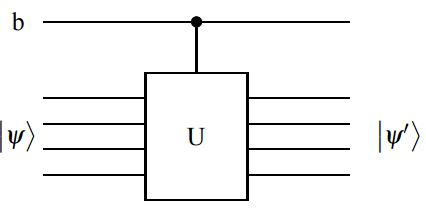
\includegraphics[scale = 0.6]{2.JPG}
    \caption{"Controlled U" Circuit}
    \label{fig:my_label}
\end{figure}
Here are the steps for the phase estimation algorithm:
\begin{enumerate}
    \item Apply a hadamard gate on the first qubit, creating an equal superposition of the basis states.
    
    \item Apply the C-U gate, encoding the eigenvalue onto the first qubit.
    
    \item Apply a hadamard gate to encode the phase into the amplitude.
    
    \item Measure the first qubit in the standard basis to estimate $\theta$.
\end{enumerate}

Summary:
\[\ket{0}\ket{\psi} \xrightarrow{\text{H}} \frac{1}{\sqrt{2}}(\ket{0} + \ket{1})\otimes\ket{\psi}\xrightarrow{\text{C-U}} \frac{1}{2}(\ket{0} + \lambda\ket{1})\otimes\ket{\psi}\xrightarrow{\text{H}}(\frac{1+\lambda}{\sqrt{2}}\ket{0} + \frac{1-\lambda}{\sqrt{2}}\ket{1})\otimes\ket{\psi}\]

The phase estimation circuit is shown:

\begin{figure}[H]
    \centering
    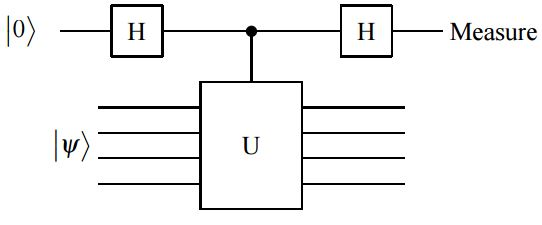
\includegraphics[scale = 0.6]{3.JPG}
    \caption{Phase Estimation Circuit}
    \label{fig:my_label}
\end{figure}

When we measure the first qubit, the probability that we see a 0 or 1 is:

\[P(0)=\left|\frac{1 + cos2\pi\theta + isin2\pi\theta}{\sqrt{2}}\right|^2 = \frac{1+cos2\pi\theta}{2}, P(1)=\left|\frac{1 - cos2\pi\theta - isin2\pi\theta}{\sqrt{2}}\right|^2 = \frac{1-cos2\pi\theta}{2}\]

If we repeat this algorithm several times, we can estimate $\theta$. However, if we want to estimate $\theta$ with m-bits of precision, we would need to perform at least $\Omega(2^m)$ iterations of the algorithm. We can speedup the algorithm with a few assumptions\cite{vaz}.

\subsection{Efficient Phase Estimation Algorithm}

In efficient phase estimation, we want to estimate $\theta$ with m-bits of precision. This is equivalent to estimating an integer $j$, where $j/2^m$ is the closest approximation to $\theta$. Let $M=2^m$and $\omega_M=e^{\frac{2\pi i}{M}}$. Assume that a k-Controlled U ($C_k-U$) circuit exists, which applies the transformation $\ket{k}\otimes\ket{\psi} \rightarrow \ket{k} \otimes U^k\ket{\psi}$.

% https://people.eecs.berkeley.edu/~vazirani/s07quantum/notes/phase.pdf

Here are the steps for the efficient phase estimation algorithm:

\begin{enumerate}
    \item Apply a $H^{\otimes m}$ on m control qubits, creating an equal superposition of the m-bit basis states.
    
    \item Apply the $C_m-U$ gate to the m-bit superposition, adding a phase to each state in the m-bit superposition. This returns a pure fourier state mod M of j.
    
    \item Apply the $QFT_M^{-1}$ to return one of the basis states, $\ket{j}$.
    
    \item Measure it in the standard basis.
\end{enumerate}

Summary:
\[\ket{0^{m}} \ket{\psi} \xrightarrow{\text{$H^{\otimes m}$}} \left(\frac{1}{\sqrt{M}}\sum_{k=0}^{M-1}\ket{k}\right)\otimes\ket{\psi}\xrightarrow{\text{$C_m-U$}} \left(\frac{1}{\sqrt{M}}\sum_{k=0}^{M-1}\lambda^k\ket{k}\right)\otimes\ket{\psi}=\left(\frac{1}{\sqrt{M}}\sum_{k=0}^{M-1}\omega_m^{jk}\ket{k}\right)\otimes\ket{\psi}\xrightarrow{\text{$QFT_M^{-1}$}} \ket{j} \otimes \ket{\psi}\]

If $\theta=j/2^m$, the algorithm will output j. If $\theta \approx j/2^m$, the algorithm will output j with high probability. If we assume that the $C_m-U$ circuit exists and has a constant run-time, the efficient phase estimation algorithm is $O(m^2)$ (dominated by the run-time of $QFT_M^{-1}$ gate). The circuit for efficient phase estimation is shown below\cite{vaz}:

\begin{figure}[H]
    \centering
    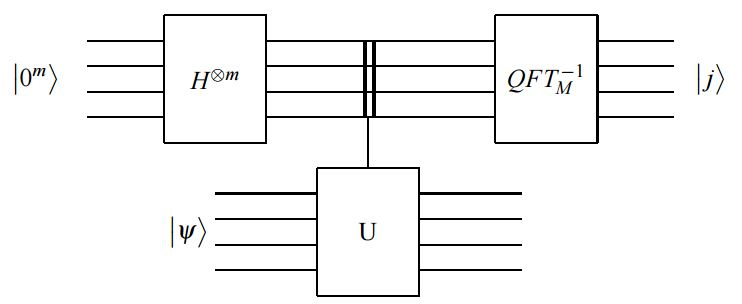
\includegraphics[scale = 0.5]{4.JPG}
    \caption{Efficient Phase Estimation Circuit}
    \label{fig:my_label}
\end{figure}

\section{Using Phase Estimation to Implement QFT$_M$}
Following lecture notes from Vazirani\cite{vaz}, we can implement the operation
\[\ket{a} \ket{0} \rightarrow \ket{0} \ket{\chi_a}, \quad \ket{\chi_a} \equiv QFT_M \ket{a},\]
given a $k$-times controlled phase shift circuit, which maps 
\[\ket{a} \ket{b} \rightarrow \omega_M^{ab} \ket{a} \ket{b}, \quad \omega_M = \exp(2 \pi i/M)\]
and a phase estimation circuit. The process consists of three steps: (1) preparing a uniform superposition over states $\ket{0}, ... \ket{M}$ on the second register, (2) performing the controlled phase shift, and (3) erasing/unentangling (with reverse phase estimation) on the first register to allow for superpositions of the second register.\\

The first step can be achieved by using a $2^n$-dimensional Hadamard circuit, where $M < 2^n$. Let $n$ bits be on the first register, with an ancilla bit, which will encode the boolean value $f(x) = (x < M)$ (which can be efficiently implemented classically, and thus quantum-ly). After computing the boolean, we measure the ancilla bit, and with probability $\geq 1/2$ measure $\ket{0}$, leaving us in the desired superposition,
\[\ket{0^n} \ket{0} \rightarrow {1\over \sqrt{2^n}} \sum_j \ket{j} \ket{0} \rightarrow {1\over \sqrt{2^n}} \sum_{j = 0}^{2^n} \ket{j} \ket{j < M}\Rightarrow {1 \over \sqrt{M}} \sum_{j = 0}^{M - 1} \ket{j}, \quad wp \geq 1/2.\]

Next, we use the first register to control the phase shift on this uniform superposition created above, and our state is 
\[\ket{a} \sum_{j=0}^{M-1} \omega_M^{aj} \ket{j}.\]
Note that the second register is the desired $\ket{\chi_a}$. However, we need to erase the first register. From lecture, we recall the effect of a constant shift $\ket{x} \rightarrow \ket{x + a}$ in the computational basis corresponds to a phase shift of $\exp(2 \pi i a/ M)$ in the Fourier basis. Recalling that the phase estimation transfers the phase of the eigenvector to the first register, i.e. 
\[\ket{0} \ket{\chi_a} \rightarrow \ket{a} \ket{\chi_a},\]
we simply run phase estimation in reverse to erase the first register, leaving us in the desired state. 

\section{Hidden Subgroup Problem (HSP)}
Many problems covered in this paper (and in class) can be generally formulated in the language of abelian groups, e.g. Simon's Algorithm, order finding, computing the discrete logarithm, etc. Many of the definitions/terminology used can be found in any standard introductory text on group theory, such as Gallian's \textit{Contemporary Abstract Algebra}. There is no known classical algorithm which can generally solve the HSP efficiently, but quantum computing provides a general method to solve in O(poly $\log M$) time, for a group of order $M$\cite{mp}.

We define a hidden subgroup $H$ of group $G$, by the function (also sometimes called an oracle) $f: x \in G \rightarrow S$ (for some finite set $S$)
\[f(x) = f(y) iff (x-y) \in H.\]
Reference \cite{mp} details a method which the generators of $H$ can be efficiently found, which is beyond the scope of this paper. Instead, we list several examples of HSPs and the group and hidden subgroup structure behind them, in the figure below. In essence, the idea is that one can generally define a Fourier transform for any finite abelian group, and using Schur orthogonality (a theorem from character theory of such groups) we ensure that the Fourier transform only keeps the terms which provide useful information on classifying $H$, while the other terms destructively interfere and vanish.\\
\begin{figure}
    \centering
    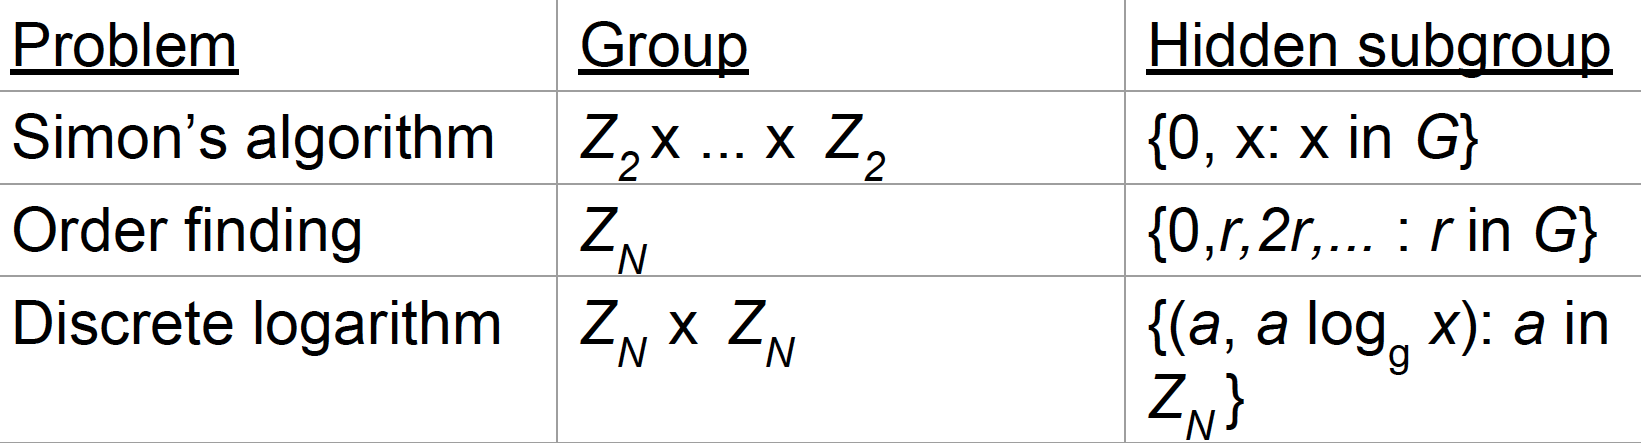
\includegraphics[scale = 0.3]{6.png}
    \caption{Examples Hidden Subgroup Problems, $Z_N$ is the group corresponding to addition of integers mod N}
\end{figure}

\section{Applications}
\subsection{Discrete Logarithm}
The Diffie-Hellman key exchange protocol is based on the assumption that the discrete logarithm on a cyclic group $G$ generated by element $g$ is difficult to compute, i.e. to find $L$ such that $g^L = x$ for any element $x \in G$. However, quantum computing may pose a threat to this protocol, as this is can be formulated as an HSP where the oracle is $f(a,b) = x^ag^b = g^{aL + b}$, and we run the algorithm by first computing in the second register
\[\sum_{a,b}\ket{a',b',0} \rightarrow \sum_{a,b}\ket{a,b,g^{aL + b}}\]
then measuring the second register to obtain a uniform superposition where $aL + b = c$, a constant. We then run the generalized QFT, given by $QFT_M \otimes QFT_M$, where $|G| = M$, which allows us to find $kL, k'L$ for coprime $k,k'$ (with good probability). A more detailed derivation can be found in \cite{mp}. 


\subsection{Order Finding}
We can use phase estimation to solve the order finding problem. For two positive integers $a$ and $N$ such that $a < N$ and $N$ is a n-bit number. We want to find the smallest positive integer $r$ such that $a^r = 1$(mod $N$). Classically, there is no known algorithm for solving this problem in polynomial time. However, using quantum computing, we can reduce the order finding problem to a specific case of phase estimation. Vazirani's CS294-2 Spring 2009 notes \cite{vaz} details the algorithm.

Recall the algorithm for phase estimation. We want to apply the operator $M_a: \ket{x} \rightarrow \ket{xa mod N}$. The eigenvectors are $\ket{\psi_k} = \frac{1}{\sqrt{r}}(\ket{1} + w^{-k}\ket{a} + ... + w^{-k(r-1)}\ket{a^{r-1}}$, where $w = e^{2\pi i/r}$. It follows that:

\[M_a = \frac{1}{\sqrt{r}}(\ket{a} + w^{-k} \ket{a^2} + ... + w^{-k(r-1)}\ket{a^{r}}) = w^k \frac{1}{\sqrt{r}} (\ket{1} + w^{-k}\ket{a} + ... + w^{-k(r-1)}\ket{a^{r-1}}) = w^k \ket{\psi_k}\]

We've effectively decomposed $M_a$ into an eigenstate, $\ket{\psi_k}$, and eigenvalue, $w^k$. Using phase estimation, we can approximate $\theta$ and reconstruct $r$, since $w^k = e^{2\pi i \theta}$ for $\theta = k/r$. For this, we will need a $C_m-M_a$ gate that transforms $\ket{k}\ket{x} \rightarrow \ket{xa^k mod N}$. Since efficient phase estimation returns a $j$ such that $\theta \approx j/2^m$, we would need to choose $M$, where $M = 2^m$, such that $M \approx N^2$ (assuming $k$ is relatively prime to $r$). Using the continued fraction algorithm, which given a fraction returns a rational number to a finite precision, we can estimate $r$. Note that $C_m-M_a$ performs modular exponentiation. The quantum order finding circuit is shown below:

\begin{figure}[H]
    \centering
    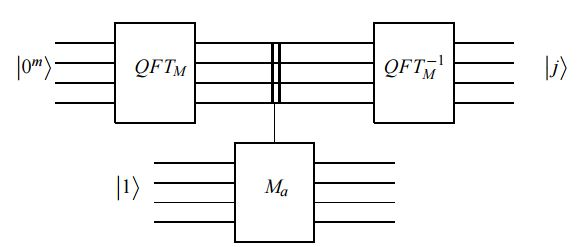
\includegraphics[scale = 0.6]{5.JPG}
    \caption{Order Finding Circuit (Kitaev's)}
    \label{fig:my_label}
\end{figure}

Here are the steps for Kitaev's order finding algorithm:

\begin{enumerate}
    \item Apply $QFT_M$ (or $H^{\otimes m}$)  to obtain an equal superposition of the m-bit basis states.
    \item Apply the $C_m-M_a$ circuit to the second qubit, $\ket{1}$, to perform the modular exponentiation over the m-bit basis states. Note that $\frac{1}{\sqrt{r}}\sum_{k=0}^{r-1} \ket{\psi_k} = \ket{1}$. Using $\ket{1}$ will allow us to measure a random eigenvalue $w^k$, where $k \in \{0,...,r-1\}$ and chosen uniformly at random. $k$ will be relatively prime to $r$ with reasonable probability.
    \item Apply $QFT_M^{-1}$ to return one of the basis states, $\ket{j}$.
    \item Measure it in the standard basis and use the continued fraction algorithm to estimate $r$.
\end{enumerate}

The circuit outputs $\ket{j}$ with high probability, where $j/2^m \approx k/r$ for some random and likely prime k. With this information, we can solve for $r$. Kitaev's order finding algorithm takes $O(n^3)$ time, for a n-bit number $N$. Michael Nielsen's and Isaac Chuang's $\textit{Quantum Computation and Quantum Information}$ describes the order finding problem and its relation to phase estimation in greater detail \cite{book}. 

\subsection{Factorization}
We saw in the previous section that if we have a periodic function f(x) = f(x+r), it was possible to recover r, the period or order, by using phase estimation to find a state $\ket{j}$ such that $j/2^m \approx k/r$, which can help us solve for r using continued fractions. 
\\\indent Factorization algorithms highlight the importance of order finding, which is motivated by phase estimation, and are incredibly relevant for usage in quantum cryptography. Shor’s and Kitaev's algorithm attempt to factor a number N into prime factors P and Q (or if the factors are not prime, they can be further reduced). Kitaev's approach generalizes Shor's attempt by utilizing phase estimation and modular exponentiation. It does this by following similar steps of the order finding algorithm \cite{factor}. First, we hope to find a number $y^2 - 1$, such that when N divides it, it yields a remainder of 0. We then could find the roots of $y^2 - 1\equiv 0 mod N$, and take the the greatest common divisor (gcd) between the roots and N to find nontrivial factors of N. To do this, we set y = $x^\frac{r}{2}$, and attempt to find r, the period of function f(a) = $x^a mod N$ for x randomly chosen between 1 and N-1.
\\\indent We apply an n-qubit Hadamard transform $\ket{0}^n$ state to yield our uniform distribution of $\ket{a}$, $\sum_a 2^{-n/2} \ket{a}$. We apply unitary transformation $U_f$ to the first 2n qubits, constructed by applying a C-U gates between $\ket{1}^n$ in the second register to the  to the first register's n qubits. This yields $2^{-n/2} \sum_a \ket{a}\ket{f(a)}$, where now we have defined f(a) = $x^a mod N$, which is a periodic function with x randomly chosen between 1 and N-1, with some probability of failure. $\ket{f(a)}$ can be reexpressed in the fourier basis of unitary transformation U, where $U\ket{u_s} = $ as $\frac{1}{\sqrt{r}} \sum_{s=0}^{r-1} e^{2\pi i as/r} \ket{u_s}$, where $\ket{u_s}$ is an eigenstate of U. Applying an inverse quantum fourier transform to the first n qubits via phase estimation and measuring the first qubit as per order finding will allow us to find s/r, and we can return r through using a continued fractions algorithm. This is beyond the scope of this paper, but essentially the output of phase estimation is $\theta = \frac{j}{2^n} \approx \frac{s}{r}$ for s being relatively prime, and using these facts to return r. This works should the number of qubits in the inverse quantum fourier transform not be a power of two. Defining $y = x^{\frac{r}{2}}$, we see that $y^2 \equiv 1 mod N$, and reexpressed, $(y^2 - 1) \equiv 0 mod N$  indicates that N is divisible by $y^2-1$. We find the nontrivial roots of $y^2 - 1 = 0$, $y_1$ and $y_2$, and can thus find two nontrivial factors of N by taking gcd($y_1$,N) and gcd($y_2$,N). The circuit is portrayed as the same figure detailing order finding, but in addition requires some classical computations\cite{vaz}.
\\\indent We see that we can use phase estimation to help us factor a number N, using $QFT_M$, when M may not be a power of two, all with a runtime of $O((log(N))^3)$ and success probability of $O(1)$. We summarize the algorithm:
    \[\ket{0}^n \overset{H_n}{\longmapsto}\sum_a\ket{a}\overset{U_f}{\longmapsto}\sum_a\ket{a}\ket{x^a mod N}=\sum_a\ket{a}\frac{1}{\sqrt{r}} \sum_{s=0}^{r-1} e^{2\pi i as/r} \ket{u_s}\overset{QFT_M^{\dagger}}{\longmapsto}\ket{\frac{s}{r}}\overset{_{Continued Fractions}}{\longrightarrow} r\]\[
    r \longrightarrow y = x^{\frac{r}{2}} \longrightarrow (y^2 - 1) \equiv 0 mod N \longrightarrow y_{Non TrivialRoot} = y_1, y_2 \longrightarrow gcd(y_1, N) = P, gcd(y_2,N) = Q\]
Shor's algorithm, as taught in class, is essentially the same as Kitaev's algorithm, but the emphasis and approach of the two algorithms are different. $\ket{0}^n$ is fed into the second register instead of $\ket{1}^n$, and Shor's realization of $U_f$ to compute the $\sum_a \ket{a}\ket{f(a)}$ differs in approach than the controlled U gates of Kitaev's, but both algorithms do the same thing. They also use QFT$_M$ for M being a power of 2 to finalize the computation (Kitaev employs the inverse). Both algorithms could revolutionize security and RSA encryption is done, though Kitaev's algorithm allows Shor's algorithm to be understood through the context of phase estimation. 

\subsection{Solving Systems of Linear Equations}
\indent A system of linear equations can be represented by A$\vec{x} = \vec{b}$. A quantum algorithm relying mostly on phase estimation can be utilized to uncover $\vec{x}$. We can each part of the linear equation with a quantum analog $A\ket{x} = \ket{b}$ where A is an NxN Hermitian matrix and A = $\sum_j \lambda_j \ket{u_j}\bra{u_j}$, where $\lambda_j$ and $\ket{u_j}$ are eigenvalues and eigenstates of A respectively, $\ket{b} = \sum_i b_i \ket{i}$ in the standard basis, and $\ket{x}$ and $\ket{b}$ both have unit length as they are quantum states\cite{sle2}. 
\\\indent We can solve this equation for $\ket{x}$ as $\ket{x}$ = $c A^{-1}$ $\ket{b}$ where $c^{-1} = || A^{-1} \ket{b} ||$. $\ket{b}$ can be reexpressed in the eigenstate basis of A as $\ket{b} = \sum_j \beta_j \ket{u_j}$, where $\beta_j = \bra{b}\ket{u_j}$. An ancillary $\ket{0}$ qubit, n computational 0 qubits ($\ket{0}^n$), and $\ket{b}$ are prepared as the input to this quantum circuit. Phase estimation (via $H^{\tens{}n}$ on $\ket{0}^n$, Hamiltonian simulation of $U = \sum_k \ket{k}\bra{k}\tens{}e^{\frac{-iA2\pi k}{2^n}}$ (roughly speaking) on the register and input, and applying $QFT_M^\dagger$ on the register) is used on $\ket{0}^n$ and $\ket{b}$ to produce $\ket{0} \sum_j \beta_j \ket{\lambda_j} \ket{u_j}$, where the quantum states representing the eigenvalues of A, $\ket{\lambda_j}$, are calculated to n-bit precision. $\ket{\lambda_j}$ results from amplitudes of fourier basis states of the solutions of $QFT_M^\dagger$ being highly concentrated about $\ket{\lambda_j}$ \cite{sle1}.
\\\indent Then, the ancillary qubit is rotated via controlled rotation gate $R(\lambda^{-1})$ (controlled by the middle register) to yield $\sum_j (\sqrt{(1-(\frac{C}{\lambda_j})^2}\ket{0} + \frac{C}{\lambda_j} \ket{1}) \beta_j \ket{\lambda_j} \ket{u_j}$, and an inverse phase estimation uncomputes the middle register back to $\ket{0}^n$, and we attain the result sum $\sum_j (\sqrt{(1-(\frac{C}{\lambda_j})^2}\ket{0} + \frac{C}{\lambda_j} \ket{1}) \beta_j \ket{0}^n \ket{u_j}$. If we measure the first/ancillary qubit and filter out all results that are not state $\ket{1}$, we get $\ket{1}\ket{0}^n\sum_j \frac{CB_j}{\lambda_j}\ket{u_j}$, where $\sum_j\frac{\beta_j}{\lambda_j}\ket{u_j}$ is simply $cA^{-1}\ket{b} = \ket{x}$, yielding our final state proportional to $\ket{1}\ket{0}^n\ket{x}$. We see that by applying a phase estimation algorithm (PE), a controlled rotation gate on the ancillary qubit, an inverse phase estimation on the bottom two registers, and selectively measuring the ancilla qubit for $\ket{1}$ (M(1) operation), we can recover a final state that is proportional to $\ket{x}$, allowing us to solve the system of linear equations A$\vec{x}$ = $\vec{b}$. A circuit diagram for the algorithm has been pictured below \cite{sle2}. 
\begin{figure}[H]
    \centering
    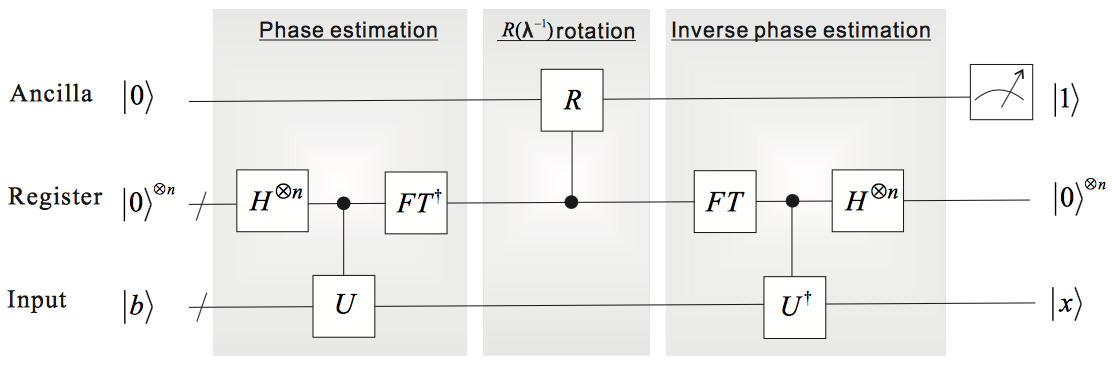
\includegraphics[scale = 0.6]{1.png}
    \caption{Quantum Solving of System of Linear Equations Algorithm}
    \label{fig:my_label}
\end{figure}
We can summarize this circuit with unitary operator $U_t$ that performs the following function: $U_t\ket{0}\ket{0}^n\ket{b} = \ket{1}\ket{0}^n\ket{x}$ via the following transformations:
 \[\ket{0}\ket{0}^n\ket{b} \overset{PE}{\longmapsto} \ket{0} \sum_j \beta_j \ket{\lambda_j} \ket{u_j} \overset{R(\lambda^{-1})}{\longmapsto} \sum_j (\sqrt{(1-(\frac{C}{\lambda_j})^2}\ket{0} + \frac{C\beta_j}{\lambda_j} \ket{1}) \ket{\lambda_j} \ket{u_j} \overset{M(1)}{\longmapsto} \sum_j  \frac{C\beta_j}{\lambda_j} \ket{1} \ket{\lambda_j} \ket{u_j} \overset{PE^{-1}}{\longmapsto} \ket{1}\ket{0}^n\ket{x}\]
What kind of resources do we expect to need for this algorithm to run and what kind of results can we expect to attain? The compute time estimated for such an algorithm is $O(\frac{log(N)s^2\kappa}{\epsilon})$ for a s-sparse NxN Hermitian matrix \cite{sle1}, where $\kappa$ is the ratio between the largest and smallest eigenvalues of A, and $\epsilon$ is the error of the output vector $\vec{x}$. Factoring in the probability of successfully selecting ancilla qubit $\ket{1}$ after the controlled $R(\lambda^{-1})$ rotation, and this compute time increases to $O(\frac{log(N)s^2\kappa^2}{\epsilon})$, which is a significant speedup over the classical algorithm, which computes the actual solution $\vec{x}$ in $O(N^3)$ runtime (gaussian elimination), and $O(N\sqrt{\kappa})$ for a summarized solution (not revealing all features of $\vec{x}$). Though $\ket{x}$ can be found in faster runtime through quantum computing than  classically finding $\vec{x}$, we are unable to determine all of the features of $\ket{x}$ unless if we recreate this scenario and remeasure $\ket{x}$ at least N times. The solution has been found more quickly than classical, but what can we know about it has been significantly reduced. To find a feature (eg. value of particular index) of $\ket{x}$, we make a measurement with observable M, with an expectation value of $\bra{x}M\ket{x}$. Running this at least N times to rebuild all features of $\vec{x}$ will increase the runtime of the total algorithm to $O(N\frac{log(N)s^2\kappa^2}{\epsilon})$, which is better than finding an exact solution classically, and the summary/sample statistic of $\vec{x}$ can be found faster using quantum computing ($O(\frac{log(N)s^2\kappa^2}{\epsilon})$ quantum compared to $O(N\sqrt{\kappa})$ classical). Knowing only a subset (brief summary) of the data may be important for calculations and simulations such as Monte Carlo simulations, which do not require the entire solution to run effectively. \\\indent Thus, phase estimation was essential in being able to produce an outcome to a nontrivial solution of a system of linear equations in compute time that is better than classical times. The phase estimation was done by turning A into a unitary $U = e^{-iAt}$ through a Hamiltonian simulation method, if A is hermitian. If A is not, you can construct a hermitian operator out of A, and solve
\[\begin{bmatrix} 0 & A \\ A^\dagger & 0\end{bmatrix} \begin{bmatrix}0\\\vec{x} \end{bmatrix} = \begin{bmatrix}\vec{b} \\ 0 \end{bmatrix}\]
using the same method. This requires runtime $O(log(N)s^2 t)$. As a potential drawbacks, the time it takes to prepare $\ket{b}$ and $e^{-iAt}$ could kill any exponential speedups over classical computing. Phase estimation is also the dominant source of error and compute time for the algorithm and generates an error bound $\epsilon$, which is introduced into our final runtime to minimize error in our solution. \cite{sle1}\cite{sle2}\cite{sle3}
%https://en.wikipedia.org/wiki/Quantum_algorithm_for_linear_systems_of_equations
%https://arxiv.org/pdf/1302.4310.pdf
%https://arxiv.org/pdf/0811.3171.pdf
%http://www.scottaaronson.com/papers/qml.pdf
%https://arxiv.org/pdf/1302.1946.pdf



% how much data we can get out of it, and error associated

\section{Conclusion}
    The hidden abelian subgroup problem has been a common theme in our C191 quantum computation class, and is a very common problem to be solved in all of quantum computation. Being able to classify a quantum computing problem as a hidden subgroup problem grossly simplifies finding its solution because there already exists a theoretical framework that is effective in handling these problems, one that utilizes QFT$_M$. In order to effectively use QFT$_M$ for generalized cases of M, the phase estimation algorithm must be used, and has been the solution algorithm to many of these subgroup problems. 
    \\\indent We have shown that the incorporation of the phase estimation algorithm in quantum computing has allowed us to solve order finding, factorization (cryptography), and discrete logarithm problems in compute times exponentially faster than their classical counterparts. Phase estimation has also been heavily used in solving systems of linear equations (machine learning, differential equations, least-squares regressions), which can prepare a solution in exponentially faster times than classical computing (though the speedup is more modest when one considers having to measure all indices of the solution to know the features of the exact result).
    \\\indent Phase estimation is a key primitive in solving many quantum computation problems, and incorporating it with the mathematical language of HSP makes it a very powerful tool for future applications.
    



\begin{thebibliography}{1} %change this

    \bibitem{mp} A. M. Childs and W. V. Dam, Reviews of Modern Physics 82, 1 (2010).

  \bibitem{factor}L.Hayes, Kitaev's Factoring Algorithm. (1997)
  
  \bibitem{vaz}Vazirani, Umesh. Vazirani’s CS294-2 Spring 2009 Lecture Notes: Lectures 5 and 6. (2009)
  
  \bibitem{book}I. L. Chuang and M. A. Nielsen, Quantum Computation and Quantum Information (2010)
  
  \bibitem{sle1}X.-D. Cai, et. al.. Experimental quantum computing to solve systems of linear equations. (2013)
  
  \bibitem{sle2}A. W. Harrow, A. Hassidim, and S. Lloyd, Quantum algorithm for linear systems of equations. (2008)
  
  \bibitem{sle3}Aaronson, Scott. Quantum Machine Learning Algorithms: Read the Fine Print (n.d.)
  
  %\bibitem
 \end{thebibliography}


\end{document}